\documentclass[main_conf.tex]{subfiles}
\begin{document}

Se diseña una caja de control (Control Box, CB) la cual cuenta
con display LCD de 16x2 y un teclado matricial de 4x4 mostradas
en la Fig. \ref{box:iso}.a habilitando una HMI. En la parte trasera
cuenta con un orificio para poder introducirle cables de poder y
lo cables conectados a un encoder para la estimación de la longitud
de la HM como se muestra en la Fig. \ref{box:iso}.b.

\begin{figure}[t]
  \centering
  \begin{subfigure}[b]{0.5\textwidth}
    \centering
    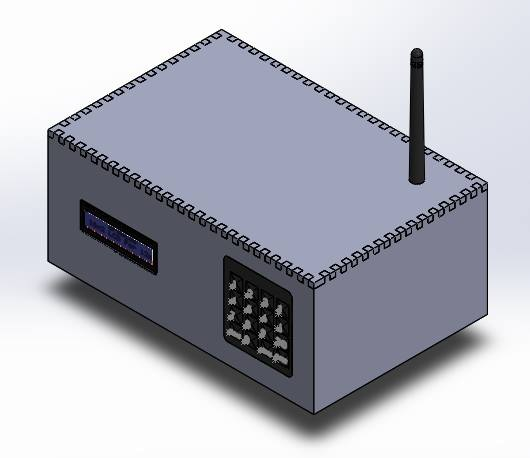
\includegraphics[width=1.5in]{../img/box/iso_front.png}
    \caption{Vista frontal}
  \end{subfigure}

  \begin{subfigure}[b]{0.5\textwidth}
    \centering
    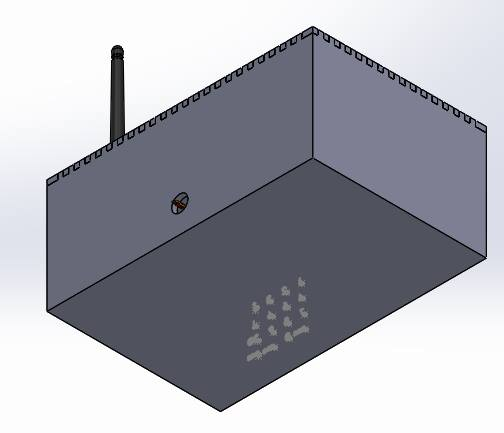
\includegraphics[width=1.5in]{../img/box/iso_back.png}
    \caption{Vista trasera}
  \end{subfigure}

  \caption{isométricas de la caja de control}
  \label{box:iso}
\end{figure}


\subsection{Modo calibración manual inicial}
Al inicio de todo el proceso es necesario una calibración manual para
alinear la hebra y ubicarla al borde de la cortadora puesto que existe
una distancia inicial entre los ruedas dentadas y la cortadora como se
muestra en la fig. \ref{distancia_inicial} con la línea roja.
Así mismo, el display LCD mostrará lo expresado en la fig.
\ref{Modo_Calibracion_manual_inicial} y esperará a que se presione
enter, transitando así al modo "estimando".

\begin{figure}[!t]
  \centering
  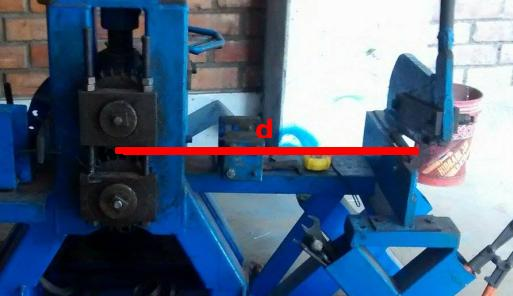
\includegraphics[width=3.0in]{../img/maquina/distancia_inicial.jpg}
  \caption{Distancia entre las ruedas dentadas y la cortadora.}
  \label{distancia_inicial}
\end{figure}

\begin{figure}[!t]
  \centering
  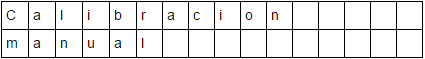
\includegraphics[width=3.0in]{../img/modo/Calibracion_manual_inicial.png}
  \caption{Texto mostrado en el modo “Calibración manual inicial”.}
  \label{Modo_Calibracion_manual_inicial}
\end{figure}

\subsection{Modo estimando}
Este es el proceso principal en el se estima la longitud de la hebra
confeccionada. Este debe ser activada sí y solo sí se ha terminado de
calibrar manualmente la posición de la hebra al inicio de la cortadora.
El formato información mostrada por el display LCD se muestra en la fig.
\ref{Modo_estimando}.a. Las variables en el formato significan:

\begin{itemize}
\item \$N: Cantidad total de hebras a confeccionar.
\item \$n: Cantidad de hebras confeccionadas hasta el momento.
\item \$L: Longitud deseada por hebra.
\item \$l: Longitud actual de la en proceso de confección.
\end{itemize}

En la fig. \ref{Modo_estimando}.b se aprecia un ejemplo con valores:
\begin{itemize}
\item $\$N = 125$
\item $\$n = 100$
\item $\$L = 15.03$
\item $\$l = 8.95$
\end{itemize}

\begin{figure}[t]
  \centering
  \begin{subfigure}[b]{0.5\textwidth}
    \centering
    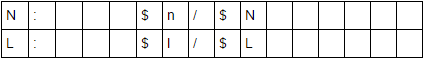
\includegraphics[width=3.0in]{../img/modo/estimando_view.png}
    \caption{Formato de texto mostrado}
  \end{subfigure}

  \begin{subfigure}[b]{0.5\textwidth}
    \centering
    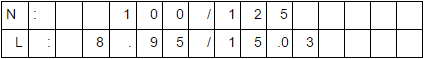
\includegraphics[width=3.0in]{../img/modo/estimando_sample.png}
    \caption{Ejemplo de texto mostrado}
  \end{subfigure}

  \caption{Formato y ejemplo del modo "estimando"}
  \label{Modo_estimando}
\end{figure}

\subsection{Modo cortadora}
Este modo indica que el operador debe hacer el corte manualmente.
En la Fig. \ref{Modo_cortadora} se mostrará el texto que
aparece en el Display LCD.

\begin{figure}[!t]
  \centering
  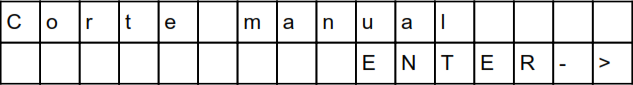
\includegraphics[width=3.0in]{../img/modo/cortadora.png}
  \caption{Texto mostrado en modo “cortadora”.}
  \label{Modo_cortadora}
\end{figure}

\subsection{Modo conf.L}
Aquí se configura la longitud de que debe tener cada HM.
En la Fig. \ref{Modo_Conf_L}.a se ve el formato a mostrar,
mientras en la Fig. \ref{Modo_Conf_L}.b se aprecia un
ejemplo con $L = 15.03$.

\begin{figure}[!t]
  \centering
  \begin{subfigure}[b]{0.5\textwidth}
    \centering
    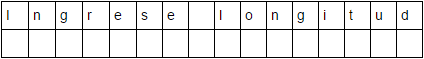
\includegraphics[width=3.0in]{../img/modo/conf_L_view.png}
    \caption{Formato de texto mostrado}
  \end{subfigure}

  \begin{subfigure}[b]{0.5\textwidth}
    \centering
    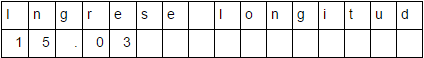
\includegraphics[width=3.0in]{../img/modo/conf_L_sample.png}
    \caption{Ejemplo de texto mostrado}
  \end{subfigure}

  \caption{Formato y ejemplo del modo "conf.L"}
  \label{Modo_Conf_L}
\end{figure}

\subsection{Modo conf.N}
Aquí se configura la longitud de que debe tener cada HM.
En la Fig. \ref{Modo_Conf_N}.a se ve el formato a mostrar,
mientras en la Fig. \ref{Modo_Conf_N}.b se aprecia un
ejemplo con $N = 1025$.

\begin{figure}[!t]
  \centering
  \begin{subfigure}[b]{0.5\textwidth}
    \centering
    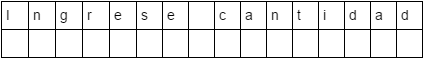
\includegraphics[width=3.0in]{../img/modo/conf_N_view.png}
    \caption{Formato de texto mostrado}
  \end{subfigure}

  \begin{subfigure}[b]{0.5\textwidth}
    \centering
    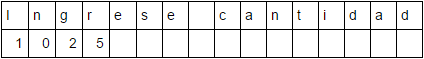
\includegraphics[width=3.0in]{../img/modo/conf_N_sample.png}
    \caption{Ejemplo de texto mostrado}
  \end{subfigure}

  \caption{Formato y ejemplo del modo "conf.L"}
  \label{Modo_Conf_N}
\end{figure}

\end{document}
